% !TeX root = document.tex
\chapter{Maschinelle Werteanpassung}

Es ist schwer menschliche Werte in Computersystemen zu programmieren (siehe Kapitel \ref{Werte}), deshalb haben \citeauthor{irving_ai_2018} einen anderen Ansatz der Werteanpassung verfolgt: die des menschlichen Feedbacks durch \emph{Deep reinforcement learning} (DRL, dt. \emph{mehrschichtiges bestärkendes Lernen}; siehe Abbildung \ref{humanfeedbackimg}). Die folgenden drei Kapitel dienen der Erklärung von wichtigen Grundbegriffen der KI-Forschung, um die wissenschaftlichen Arbeiten von \citeauthor{irving_ai_2018} zu verstehen.

\section{Reinforcement Learning}
Reinforcement Learning (RL, dt. \emph{bestärkendes Lernen}) beschreibt ein Lernverfahren einer KI, bei der sie durch durch Erfolg und Misserfolg, durch Belohnung und Bestrafung lernt. \citeauthor{russell_artificial_2016} erklären RL zusammengefasst so: \zit[831]{russell_artificial_2016}{Imagine playing a new game whose rules you don't know; after a hundred or so moves, your opponent announces, \enquote{You lose.} This is reinforcement learning in a nutshell.}

Die Aufgabe von RL ist es, wahrgenommene Belohnungen und Bestrafungen zu benutzen, um die optimale Verfahrensweise (eng. \emph{policy}) in einer gegebenen Umgebung zu finden. Dabei hat die KI a priori kein Wissen über ihre Umgebung oder Nutzfunktion. Die Nutzfunktion, definiert über Umgebungszustände, zeigt dabei den Nutzen einer bestimmten Verfahrensweise. Die optimale Verfahrensweise ist diejenige, die den höchsten erwarteten Nutzen bringt.

RL wird in Bereichen eingesetzt, in denen es nicht genug Daten gibt, oder in denen es nicht lohnenswert ist, die notwendige Menge an Daten zu verarbeiten, um eine KI auf alle möglichen Umgebungszustände vorzubereiten. Eine KI, die beispielsweise versucht, Schach zu lernen, müsste $10^{120}$ (auch Shannon-Zahl genannt) verschiedene Schachspiele gesehen haben, um allein anhand von Beispielen auf jede Situation vorbereitet zu sein. \vgl[4]{shannon_programming_1988} Bei RL vermittelt man der KI stattdessen, wann sie gewonnen oder verloren hat. Sie sucht dann auf Basis dieser Informationen eine Funktion, die die Gewinnwahrscheinlichkeit jeder gegebenen Position einigermaßen akkurat einschätzt.
\vgl[830-831]{russell_artificial_2016}

\section{Deep learning}
Deep Learning (DL, dt. \emph{mehrschichtiges Lernen}) ist ein Teilbereich des maschinellen Lernens. Dabei versucht eine KI Inputdaten mit Hilfe von Hierarchien von Konzepten zu verstehen. Der Grundansatz von DL ist das Verstehen von komplexen Konzepten durch Kombinieren von einfacheren Konzepten. \vgl[1-8]{Goodfellow-et-al-2016} Diese Konzeptschichten werden in DL fast immer mit Hilfe von künstlichen neuronalen Netzen (KNN, engl. \emph{artificial neural network, ANN}) gelernt. \vgl[8]{manning_unknown_deep_2017}



\begin{figure}
  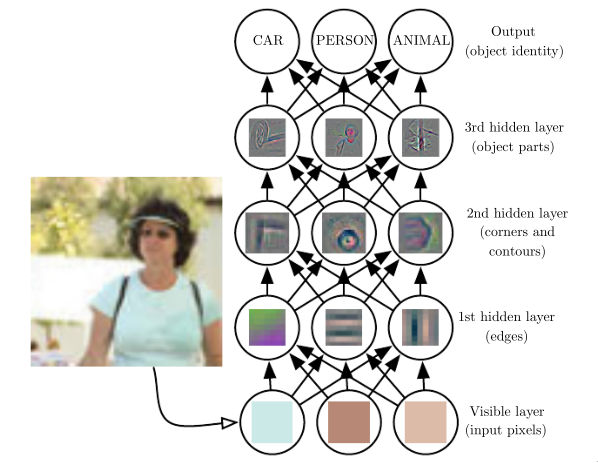
\includegraphics[width=\textwidth]{deeplearning}
  \caption{Veranschaulichung eines DL-Modells. Die KI bekommt rohe Pixeldaten als Input. Mit jeder Schicht wendet sie ein neues Konzept auf das vorherige an, die Konzepte sind also aufbauend.  \bildquelle[6]{Goodfellow-et-al-2016}}
  \label{deeplearningimg}
\end{figure}
\section{Deep reinforcement learning}

Deep reinforcement learning

\section{Deep reinforcement learning von menschlichen Werten}

\section{KI-Sicherheit durch KI-Debatten}

Hierbei fragt eine KI einen menschlichen Operator nach der Nützlichkeit und Sicherheit ihres Verhaltens. Bei schlechter Bewertung passt die KI ihre Lösungsfunktion an, somit ist weder eine Werteprogrammierung, noch eine riskante Zielsetzung im Vorhinein notwendig. \vgl{christiano_deep_2017} Dies funktioniert so lange gut, bis der Operator nicht mehr in der Lage ist, das Handeln der KI nachzuvollziehen und zu beurteilen. \vgl[1-2]{irving_ai_2018}

\begin{figure}
  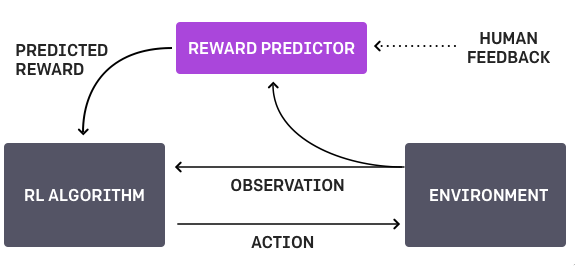
\includegraphics{humanfeedback}
  \caption{Repräsentation einer human-feedback-loop}
  \label{humanfeedbackimg}
\end{figure}

\section{AI Safety via Debate}
\section{Inverse Reward Design}

%Was ist eine Reward function?
%Eine Nutzfunktion ist 


%Ein Algorithmus einer sicheren AKI muss die folgenden Probleme lösen:
%\begin{enumerate}
%\item Negative Effekte durch eine fehlerhaft definierte Nutzfunktion zur Feststellung der Ziele
%\item Eine AKI könnte eine Problemstellung mit der Intention, sie wieder lösen zu können, verschlimmern. (Ein Staubsaugroboter, der Staub herstellt, um ihn dann wieder aufsaugen zu können.) \vgl[1-2]{hadfield-menell_inverse_2017}
%\end{enumerate}

%https://80000hours.org/articles/ai-safety-syllabus/
%\vgl{yudkowsky_intelligence_2013}
%\section{Wertekodierung in einer Programmiersprache}
%KOMMENTAR: Complexity of Value Theory
%\subsection{Statische Wertekodierung}
%\subsection{Dynamisch-maschinelle Werteanpassung}
%
%\section{Mensch-Maschinen-Interface}
%\section{Hirnemulation}
%\section{Friendly AI}



%%% Local Variables:
%%% mode: latex
%%% TeX-master: "document"
%%% End:
